%!TEX root = ./main.tex

\section{THEORY}\label{sec:theory}
%%%%%%%%%%%%%%%%%%%%%%%%%%%%%%%%%%%%
\subsection{Coordinate Descent for SLOPE}%
\label{sec:coordinate-updates}

Proximal coordinate descent cannot be applied to \Cref{pb:slope} because it is not separable.
However, if the clusters $\mathcal{C}_1^*, \ldots, \mathcal{C}_{m^*}^*$ of the solution $\beta^*$ were known together with $\sign()\beta^*)$, then the values $c_1^*, \ldots, c_{m^*}^*$ taken by $\beta^*$ on the clusters could be equivalently computed by solving:
\begin{problem}
  \begin{multlined}
  \min_{z \in \bbR^{m^*}}\bigg(
    \frac{1}{2n} \Big\lVert y - X \sum_{i=1}^{m^*} \sum_{j \in \mathcal{C}_i^*} z_i \sign(\beta_j^*) e_j \Big\rVert^2 \\
    + \sum_{i=1}^{m^*} | z_i | \sum_{j \in \mathcal{C}_i^*} \lambda_j
   \bigg).
  \end{multlined}
\end{problem}
% \klopfe{Clarify what $F$ is here}
% MM: removed F and used the form (ell(beta) instead of F(Xbeta)) : more general
% where $\tilde{x}_{\mathcal{C}_i} = \sum_{j \in \mathcal{C}_i} x_j \sign (\beta_j^*)$.
Conditionally on the knowledge of the clusters and the signs of the coefficients, the penalty becomes separable as shown by \cite{dupuis2021}, and coordinate descent could be used.
Hence, the idea of our algorithm is to intertwine steps that allows the clusters to split, and large coordinate-wise steps on these clusters.
The combination of proximal gradient descent steps and proximal coordinate descent avoids the situation depicted in \Cref{fig:naive-cd-stuck} where coordinate descent gets stuck.


A full proximal coordinate descent is possible by examine all possible direction proposed by the directional derivative. However, for a cluster of size $k$ there will be $k$ directions that needs to be computed, and for at least a naive implementation this is computationally very demanding. So instead we alternate between proximal gradient descent, to determine the cluster components, and proximal coordinate descent, to determine the coefficients.


Based on this observation, we derive a coordinate descent algorithm for minimizing the SLOPE problem~\eqref{pb:slope} with respect to the coefficients of a single cluster at a time.

In all the sequel, $\beta$ is fixed, with $m$ clusters $\mathcal{C}_1, \ldots, \mathcal{C}_m$ corresponding to values $c_1, \ldots, c_m$.
Let also $k \in [m]$ be fixed, let $s_k = \sign \beta_{\mathcal{C}_k}$.
We are interested in updating $\beta$ by changing only the value taken on the $k$-th cluster.
To this end, we let
\mm{$s_k$ issue below}
\begin{equation}
  \label{eq:coordinate-update-beta}
  \beta_i(z) =
  \begin{cases}
    s_k z   \, , & \text{if } i \in \mathcal{C}_k \, , \\
    \beta_i \, , & \text{otherwise} \, .
  \end{cases}
\end{equation}
% This means that \(\beta(z)\) corresponds to a version of \(\beta\) with a
% coordinate update for the \(k\)-th cluster.
Minimizing the objective in this direction amounts to solving the following
one-dimensional problem:
\begin{problem}
\label{pb:cluster-problem}
\min_{z \in \mathbb{R}} \Big(
G(z) = P(\beta(z))  = \frac{1}{2 n} \norm{y - X \beta(z)}^2 + H(z)
\Big) \,  ,
\end{problem}
where
\[
  H(z) = |z| \sum_{j \in \mathcal{C}_k} \lambda_{(j)^-_z}
  + \sum_{j \notin \mathcal{C}_k} |\beta_j| \lambda_{(j)^-_z}
\]
is the \emph{partial sorted \(\ell_1\) norm} with respect to the \(k\)-th cluster and where we write \(\lambda_{(j)^-_z}\) to indicate that the inverse sorting permutation \((j)^-_z\)
is defined with respect to \(\beta(z)\).
The optimality condition for \Cref{pb:cluster-problem} is
\[
  % P_k'(z; \delta) \geq 0,
  \forall \delta \in \{-1, 1\}, \quad G'(z; \delta) \geq 0,
\]
where $G'(z; \delta) $ is the directional derivative of $G$ in the direction $\delta$.
Since the quadratic datafit is differentiable we have
\[
  G'(z; \delta)  = \delta \sum_{j \in \mathcal{C}_k} X_{:j}^\top(X\beta(z) - y) + H'(z; \delta) \, ,
\]
where \(H'(z; \delta)\) is the directional derivative of $H$.

Throughout the rest of this section we derive the solution to \eqref{pb:cluster-problem}.
To do so, we will introduce the directional derivative for the
sorted \(\ell_1\) norm with respect to the coefficient of the \(k\)-th cluster.
First, as illustrated on \Cref{fig:partial_slope}, note that $H$ is piecewise affine, with breakpoints at 0 and all $\pm c_i$'s for $i \neq k$.
Hence, the partial derivative is piecewise constant, with jumps at these points; in addition, $H'(\cdot; 1) = H'(\cdot, -1)$ except at these points.

\begin{figure}[htbp]
  \centering
  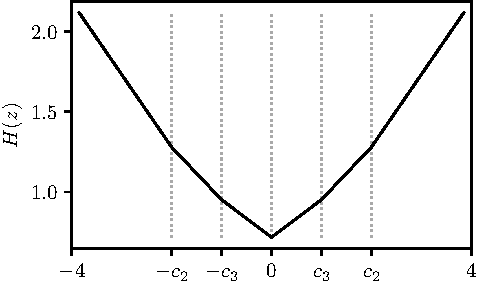
\includegraphics[width=\linewidth]{partial_slope.pdf}
  \caption{Graph of the partial sorted $\ell_1$ norm with \(\beta = [-3.0, 1.0, 3.0, 2.0]^T\), \(k = 1\), and so $c_1, c_2, c_3 = (3, 2, 1)$.}
  \label{fig:partial_slope}
\end{figure}

Let \(C(z)\) be the function that returns the cluster of $\beta(z)$ corresponding to \(|z|\), that is
\begin{equation}
  C(z) = \{j : |\beta(z)_j| = |z|\} \,.
\end{equation}



\begin{remark}\label{rem:permutation_C_z}
  Note that, if $z$ is equal to some $c_i$ then $C(z) = \mathcal{C}_i \cup \mathcal{C}_k$ and otherwise $C(z) = \mathcal{C}_k$.
  Related to the piecewise affineness of $H$ is the fact that the permutation\footnote{the permutation is in fact not unique, without impact on our results. This is discussed when needed in the proofs.} corresponding to $\beta(z)$ is:
  % \mm{there are multiple possible permutations in fact, this matters when $|z| = c_i$}
  \begin{equation*}
    \begin{cases}
    \cC_k, \cC_m, \ldots, C_1 \, ,
        &\text{ if } z \in \left]0, c_m\right[ \, \\
    \cC_m, \ldots ,\cC_i, \cC_k, \cC_{i-1}, \ldots, C_1 \, ,
        &\text{ if } z \in \left]c_{i}, c_{i-1} \right[, \, i \in \llbracket 2 , m \rrbracket \, \\
    \cC_m, \ldots C_1,  \cC_k \, ,
        &\text{ if } z \in \left]c_1, +\infty \right[ \, , \\
    \end{cases}
  \end{equation*}
  and that this permutation also reorders $\beta(z \pm h)$ for $z \neq c_i \; (i \neq k)$ and $h$ small enough.
  The only change in permutation happens when $z = 0$ or $z = c_i \; (i \neq k)$.
  Finally, the permutations differ between $\beta(z + h)$ and $\beta(z - h)$ for arbitrarily small $h$ if and only if $z = c_i \neq 0$.
\end{remark}

% Then for \(\delta \in \{-1, 1\}\) we have
% \begin{equation}
%   \begin{aligned}
%     \lim_{h \downarrow 0} C(z + h\delta)
%           & = C(z + {\varepsilon_c} \delta) \, ,  \\
%     \lim_{h \downarrow 0} \lambda_{(i)^-_{z + h\delta}}
%           & = \lambda_{(i)^-_{z + {\varepsilon_c}\delta}} \, .
%   \end{aligned}
% \end{equation}
% \mm{nitpick: permutations are not unique because of potential ties, so the second limit may not be true if ties are not handled consistently. We can say when we introduce the sorting that we break ties by picking the lowest index}
% In other words, the order permutation corresponding to \(\beta(z + h\delta)\)
% depends only on \(\delta\) as \(h\) tends to~\(0\).
% \begin{remark}
%   As consequence of the definition of \(\varepsilon_c\), the order permutations
%   for \(\beta(z)\) and \(\beta(z + {\varepsilon_c} \delta)\) differ only for a
%   subset of the permutation vectors.
%   The permutation for \(\beta(h\delta)\) is %\mm{for $h \neq 0$, but if equal to 0, two clusters merge}
%   \begin{equation*}
%     \begin{cases}
%       \mathcal{C}_1, \dots, \mathcal{C}_{k-1}, \mathcal{C}_{k+1}, \dots, \mathcal{C}_m, C(\varepsilon_c)
%        & \text{if } c_m > 0 \, , \\ % \text{ and } \delta \neq 0 \, , \\
%       \mathcal{C}_1, \dots, \mathcal{C}_{k-1}, \mathcal{C}_{k+1}, \dots, C(\varepsilon_c), \mathcal{C}_m
%        & \text{if } c_m = 0 \, . %\text{ and } \delta \neq 0 \, . \\
%       % \mathcal{C}_1, \dots, \mathcal{C}_{k-1}, \mathcal{C}_{k+1}, \dots, \underbrace{\mathcal{C}_k \cup \mathcal{C}_m}_{C({\varepsilon_c}\delta)} & \text{if } c_m = 0 \text{ and } \delta = 0.    \\
%     \end{cases}
%   \end{equation*}
%   If \(z \neq 0\), the permutation for \(\beta(z + {\varepsilon_c} \delta)\) corresponds to
%   \[
%     \begin{cases}
%       \splitfrac{\mathcal{C}_1, \dots, \mathcal{C}_{k-1}, \mathcal{C}_{k+1}, \dots, }{C(c_i + {\varepsilon_c}\delta), \mathcal{C}_k, \dots, \mathcal{C}_m} & \text{if } \delta = 1 \,,   \\
%       \splitfrac{\mathcal{C}_1, \dots, \mathcal{C}_{k-1}, \mathcal{C}_{k+1}, \dots,}{ \mathcal{C}_k, C(c_k + {\varepsilon_c}\delta), \dots, \mathcal{C}_m} & \text{if } \delta = -1 \, . \\
%       % \mathcal{C}_1, \dots, \mathcal{C}_{k-1}, \mathcal{C}_{k+1}, \dots, \underbrace{\mathcal{C}_i \cup \mathcal{C}_k}_{C(c_i + {\varepsilon_c}\delta)}, \dots, \mathcal{C}_m & \text{if } \delta = 0.  \\
%     \end{cases}
%   \]
%   \mm{I don't get why $\mathcal{C_k}$ appears with $C$, isn't it contained in $C$ ?}
% \end{remark}
%, defined as
% \(c^{(k)} = \{c_1, c_2, \dots, c_m\} \setminus c_k\), such that
% \[
%   c_i^{(k)} =
%   \begin{cases}
%     c_i     & \text{if } i < k,    \\
%     c_{i+1} & \text{if } i \geq k.
%   \end{cases}
% \]

We can now state the directional derivative of $H$. % \(J_k\).

\begin{theorem}\label{thm:sl1-directional-derivative}
  Let \(c^{\setminus k}\) be the set containing all elements of $c$ except the $k$-th one: $c^{\setminus k} =  \{c_1, \ldots c_{k-1}, c_{k+1}, \ldots, c_m \}$.
  % Let $\varepsilon_c$ be an arbitrary positive value such that
  Let $\varepsilon_c > 0$ such that
  \begin{equation}
    \label{eq:epsilon-c}
    \varepsilon_c < \big| c_i - c_j\big| , \quad \forall\, i \neq j \text{ and } \varepsilon_c < c_m \text{ if } c_m \neq 0 \, .
  \end{equation}
  The directional derivative of the partial sorted $\ell_1$ norm with respect to the $k$-th cluster, \(H\), in the direction \(\delta\) is
  \[
    H'(z; \delta) =
    \begin{cases}
      \smashoperator[r]{\sum_{j \in C(\varepsilon_c )}} \lambda_{(j)^-_{\varepsilon_c }}
       & \text{if } z = 0 \, ,               \\
      \sign(z)\delta\smashoperator{\sum_{j \in C(z + {\varepsilon_c} \delta)}} \lambda_{(j)^-_{z + {\varepsilon_c}\delta}}
      %  & \text{if } |z| = c^{(k)}_i > 0 \, , \\
       & \text{if } |z| \in c^{\setminus k} \setminus \{0\} , \\
      \sign(z)\delta\smashoperator{\sum_{j \in C(z)}} \lambda_{(j)^-_{z}}
       & \text{otherwise} \, .
    \end{cases}
  \]
\end{theorem}
The proof is in \Cref{app:proof_directional_slope}; in \Cref{fig:directional-derivative}, we show an example of the directional
derivative and the objective function.

\begin{figure}[htb]
  \centering
  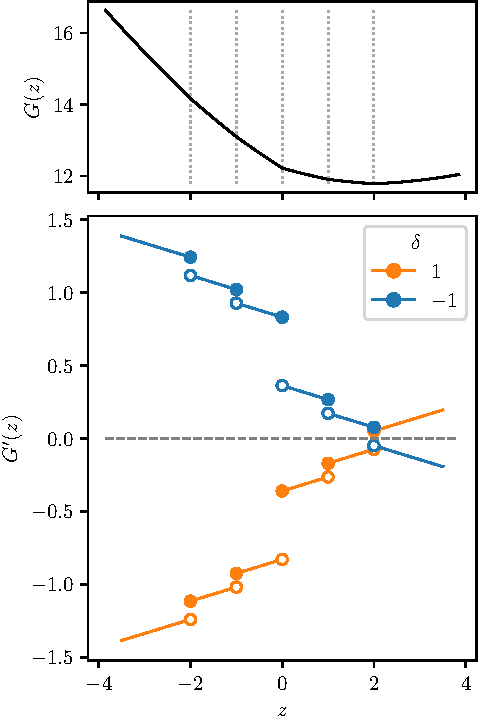
\includegraphics[]{directional-derivative.pdf}
  \caption{%
  The function \(G\) and its directional derivative \(G( \cdot ; \delta)\) for
  an example with \(\beta = [-3.0, 1.0, 3.0, 2.0]^T\), \(k = 1\), and consequently
  \(c^{\setminus k} = \{1, 2\}\). The solution of \Cref{pb:cluster-problem} is the value of \(z\) for
      which \(G'(z; \delta) \geq 0 \) for \(\delta \in \{-1, 1\}\), which holds only
      at \(z = 2\), which must therefore be the solution.
    }
  \label{fig:directional-derivative}
\end{figure}

Using the directional derivative, we can introduce the SLOPE thresholding operator.

\begin{theorem}[The SLOPE Thresholding Operator]
  \label{thm:thresholding-operator}
  Define \(S(x) = \sum_{j \in C(x)}\lambda_{(j)^-_{x}}\) and
  let
  \[
    \begin{multlined}
      T_k(\gamma; \omega, c, \lambda) = \\
      \begin{cases}
        0
            & \text{if } |\gamma| \leq S(\varepsilon_c),               \\
        \sign(\gamma)c_i
            & \text{if } \omega c_i + S(c_i - \varepsilon_c)           \\
            & \quad \leq |\gamma| \leq                                 \\
            & \quad \omega c_i + S(c_i + \varepsilon_c),               \\
        \frac{\sign(\gamma)}{\omega} \big( |\gamma| - S(c_i + \varepsilon_c) \big)
            & \text{if } \omega c_i + S(c_i + {\varepsilon_c})         \\
            & \quad < |\gamma| <                                       \\
            & \quad \omega c_{i - 1} + S(c_{i - 1} - {\varepsilon_c}), \\
        \frac{\sign(\gamma)}{\omega} \big( |\gamma| - S(c_1 + {\varepsilon_c}) \big)
            & \text{if } |\gamma| \geq                                 \\
            & \quad \omega c_1 + S(c_1 + {\varepsilon_c}).
      \end{cases}
    \end{multlined}
  \]
  with \({\varepsilon_c}\) defined as in \eqref{eq:epsilon-c}.
  Let $\tilde x = X_{\cC_k} \sign(\beta_{\cC_k})$ and $\tilde r = y - X_{\bar \cC_k} \beta_{\bar \cC_k}$.
  Let \(\gamma = \tilde{r}^Tx\), \(\omega = \tilde{x}^T\tilde{x}\). Then
  \(T(\gamma; \omega, c^{(k)}, \lambda) \in \argmin_{z \in \mathbb{R}} G(z)\).
  Then:
  \begin{equation}
    T \left(\beta_{\cC_k} - \tfrac{1}{\Vert \tilde x \Vert^2} \tilde x (y - X\beta)); \Vert \tilde x \Vert^2, c^{\setminus k}, \lambda \right) \in \argmin_{z \in \mathbb{R}} G(z) \,.
  \end{equation}
\end{theorem}

\mathurin{add remark on uniqueness of argmin? $G(z)$ is a 1 quadratic so it's either constant (possible) either there's a single minimizer}

\begin{remark}
  In the Lasso case where the $\lambda_i$'s are all equal and $m = p$, the SLOPE Thresholding Operator is a soft thresholding operator.
\jl{Consider adding a remark showing that our operator generalizes the soft thresholding operator.}
\end{remark}

In \Cref{fig:slope-thresholding}, we visualize the SLOPE thresholding operator.

Note that it is typically not necessary to compute all partial sums in \Cref{thm:thresholding-operator}.
Instead, we need only to first check in which direction we need to search relative to the current order for the cluster and then search in that direction until we find the solution.
The complexity of this search depends on how far we need to search in order to find the solution and the size of the current cluster.
For each change in order, we need to compute a partial sum of the \(\lambda\) sequence across as many entries as there are members of the cluster.
In practice, this means that the costs involved are often large at the start of optimization but become marginal as the identity of the clusters approach the true clusters.

\jl{The text above needs refinement and more rigor.}

\begin{figure*}[htb]
  \centering
  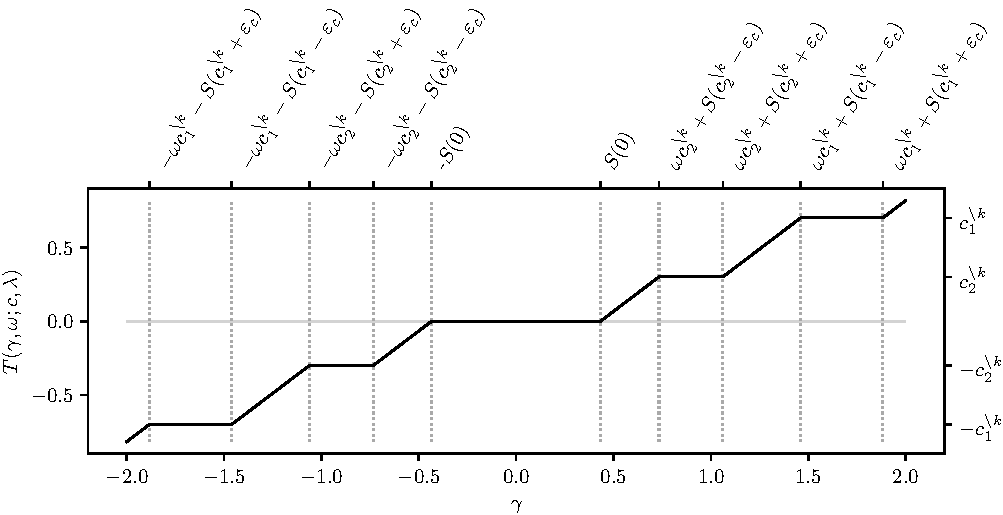
\includegraphics[]{slope-thresholding.pdf}
  \caption{%
  An example of the SLOPE thresholding operator. The result corresponds to an
  example for \(\beta = [0.5, -0.5, 0.3, 0.7]^T\), \(c = (0.7, 0.5, 0.3)\)
  with an update for the second cluster (\(k = 2\)), such that
  \(c^{\setminus k} = (0.5, 0.3)\). Across regions where the function is constant,
      the operator sets the result to be either exactly 0 or to the value of one
      of the elements of \(c^{\setminus k}\).
    }
  \label{fig:slope-thresholding}
\end{figure*}

\subsection{Hybrid Strategy}
\label{sec:hybrid-strategy}

We now present in \Cref{alg:hybrid} the proposed solver.
Every $v$ iterations, we perform a proximal gradient descent update to allows for clusters to split eventually.
The choice of the parameter $v$ that accounts for the frequency at which pgd steps are performed was set to $5$.
Our own experiments show that this parameter does not have a great impact on the speed of the algorithm as long as it is at least $3$ (see \Cref{fig:pgd_freq}).

The combination of the proximal gradient steps and PCD allows us to overcome the problem of vanilla PCD getting stuck because of non-separability and allows us to enjoy the speed-up provided by making local updates on each cluster as illustrated in \Cref{fig:illustration-solver}.

\begin{algorithm}[h!]
  \SetKwInOut{Init}{init}
  \SetKwInOut{Input}{input}
  \caption{%
    Hybrid coordinate descent and proximal gradient descent algorithm
    for SLOPE\label{alg:hybrid}}
  \Input{
    \(X \in \mathbb{R}^{n\times p}, y\in \mathbb{R}^n, \lambda \in \{\mathbb{R}^p : \lambda_1 \geq \lambda_2 \geq \cdots > 0\}\), \(v \in \mathbb{N}\)}

  \Init{\(t \gets 0\), \(\beta \gets 0\), \(L \gets \lVert X \rVert_2^2\)}

  \Repeat{convergence}{
  \(t \gets t + 1\)

  \If{\(t \bmod v = 0\)}{
    \(\beta \leftarrow \prox_{J}(\beta - \frac{1}{L}\nabla f(\beta); \lambda / L)\) \label{alg:hybrid-istastep}

    Update \(c\), \(\mathcal{C}\)
  }
  \Else{
    \(k \gets 0\)

    \While{\(k \leq \lvert \mathcal{C} \rvert\)}{
      \(k \gets k + 1\)

      \(s \leftarrow \mathrm{sign}(\beta_{\mathcal{C}_k})\)

      \(\tilde x_k \gets X_{\mathcal{C}_k}s\)

      % \(\tilde r_k \gets y - X_{\widebar{\mathcal{C}}_k}\beta_{\widebar{\mathcal{C}}_k}\)



      % \(\beta \gets T(\tilde{r}^T \tilde{x}_k; \tilde{x}_k^T \tilde{x}_k, c^{\setminus k}, \lambda)\)
      \(z \gets T(\beta - \frac{1}{\norm{\tilde x_k}^2}\tilde{x}_k^\top(y - X\beta); \tilde{x}_k^T \tilde{x}_k, c^{\setminus k}, \lambda)\)

      $\beta_{\cC_k} \gets z \sign(\beta_{\cC_k})$

      Update \(c\), \(\mathcal{C}\)
    }
  }

  }
  \Return{\(\beta\)}
\end{algorithm}

Please see \Cref{sec:computational-details} for computational details regarding the implementation of the algorithm.

\begin{figure*}[htb]
  \centering
  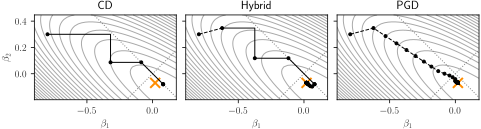
\includegraphics{illustration_solvers}
  \caption{Illustration of the proposed solver. The figures show progress
    until convergence for the coordinate descent (CD) solver that we use as part
    of the hybrid method, our hybrid method, and  proximal gradient descent
    (PGD). The orange cross marks the optimum. Dotted lines indicate where the
    coefficients are equal in absolute value. The dashed lines indicate PGD
    steps and solid lines CD steps. Each dot marks a complete epoch, which may
    correspond to only a single coefficient update for the CD and hybrid
    solvers if the coefficients flip order. Each solver was run until the duality
    gap was smaller than \(10^{-10}\). Note that the CD algorithm cannot split clusters
    and is therefore stuck after the third epoch. The hybrid and PGD algorithms,
    meanwhile, reach convergence after 67 and 156 epochs respectively.}
  \label{fig:illustration-solver}
\end{figure*}

We now state that our proposed hybrid algorithm converges to a solution of \Cref{pb:slope}.

\begin{lemma}
  \label{lem:convergence}
  Let \(\beta^{(1)}, \beta^{(2)}, \dots, \beta^{(k)}\) be a sequence of
  iterates generated by \Cref{alg:hybrid}, \(1/v\) the frequency of proximal gradient
  descent iterates in \Cref{alg:hybrid}, and \(L\) the Lipschitz constant of
  \(\nabla F\). Then
  \[
    P(\beta^{(k)}) - P(\beta^*) \leq \frac{L \lVert \beta^{(0)} - \beta^* \rVert_2^2}{2\lfloor k/v \rfloor }\, ,
  \]
  where \(\beta^* \in \argmin_{\beta \in \mathbb{R}^p} P.\)
\end{lemma}
